%Este trabalho está licenciado sob a Licença Creative Commons Atribuição-CompartilhaIgual 3.0 Não Adaptada. Para ver uma cópia desta licença, visite http://creativecommons.org/licenses/by-sa/3.0/ ou envie uma carta para Creative Commons, PO Box 1866, Mountain View, CA 94042, USA.

%\documentclass[main.tex]{subfiles}
%\begin{document}

\chapter{Integração Numérica}\index{integração}

Neste capítulo discutiremos técnicas numéricas para aproximar \emph{integrais}\index{integral} definidas de funções reais.

Considere o problema de calcular (ou estimar) a integral de $f(x)$ no intervalo $[a,b]$, ou seja,
$$
 I = \int_a^b f(x) \;dx.
$$

Uma maneira de estimar esta integral numericamente consiste em subdividir o intervalo $[a,b]$ em $n-1$ intervalos a partir de um conjunto ordenado de pontos $a=x_1<x_2<...<x_n=b$. 
Em cada intervalo $i$, a integral será aproximada por $\Delta S_i$ e a integral será aproximada por 
$$
 I \approx S = \sum_{i=1}^{n-1} \Delta S_i
$$
O tamanho de cada intervalo é dado por $h_i=x_{i+1}-x_i$. No caso uniforme, todos os intervalos possuem o mesmo tamanho $h=h_i=\frac{b-a}{n}$.

Nas próximas seções apresentaremos formas diferentes de aproximar $\Delta S_i$ iniciando com o caso mais simples que é um retângulo. Cada uma das regras obtidas também é chamada de quadratura.

\begin{ex}
A figura~\ref{fig:int_101} mostra um exemplo quando $f(x)=x^2+1$, $0\leq x\leq 2$. Temos a aproximação por um retângulo com base $h_1=2$, depois com dois retângulos de base $h_2=1$ e, finalmente com quatro retângulo de bases $h_3=0,5$.
\begin{figure}
  \centering
  \includegraphics[scale=0.7]{./cap_integracao/pics/int_1/int_1.eps}
  \caption{Aproximação por retângulos.}
  \label{fig:int_101}
\end{figure}

Os valores aproximados para a integral são dados na seguinte tabela:

\begin{tabular}{|c|c|}\hline
  & $\displaystyle \int_0^2(x^2+1)dx$ \\ \hline
  $h_1=2$ & $h_1f(1)=4$ \\
  $h_2=1$ & $h_2f(0,5)+h_2f(1,5)=4,5$ \\
  $h_3=0,5$ & $4,625$ \\
  $h_4=0,25$ & $4,65625$ \\\hline
\end{tabular}

Observe que:
\begin{equation*}
  \int_0^2(x^2+1)\,dx = \left[\frac{x^3}{3}+x\right]_0^2 = \frac{8}{3}+2=4,6666667
\end{equation*}
\end{ex}

%%%%%%%%%%%%%%%%%%%%
% python
%%%%%%%%%%%%%%%%%%%%
\ifispython
Nos códigos \verb+Python+ apresentados ao longo deste capítulo, estaremos assumindo:
\begin{verbatim}
>>> from __future__ import division
>>> import numpy as np
\end{verbatim}
\fi
%%%%%%%%%%%%%%%%%%%%



\section{Regras de Newton-Cotes}\index{integração numérica!regras de Newton-Cotes}

O método básico para encontrar as regras de integração consiste em aproximar a integral de $f$ por uma combinação linear de $n$ valores\footnote{Utilizaremos neste capítulo a notação $f_i$ para indicar $f(x_i)$.} de $f_i := f(x_i)$, ou seja,
$$
 I = \int_a^b f(x) \;dx \approx \sum_{i=1}^nA_if_i.
$$

% Quanto maior o número de pontos $n$, melhor será a regra de quadratura.

Podemos obter os coeficientes $A_i$ aproximando a função $f$ pelo polinômio de Lagrange $p_n$ que interpola $\{(x_i,f_i)\}_{i=1}^n$, tal que, 
\begin{eqnarray}
  f(x) &=& p_n(x)+E^n_{LAG}(x) \\
       &=& \sum_{i=1}^n f_iL_i(x)+E^n_{LAG}(x) 
\end{eqnarray}
onde o erro na interpolação de Lagrange é
\begin{equation}
   E^n_{LAG}(x)=\frac{f^{(n)}(\xi(x))}{n!}\prod_{i=1}^n(x-x_i).
\end{equation}

Substituindo na integral obtemos
\begin{eqnarray}
  \int_a^bf(x)dx &=& \sum_{i=1}^n\left[f_i\int_a^bL_i(x)dx\right] +  \int_a^b E^n_{LAG}(x) \;dx.
%   \int_a^bf(x)dx &=& \sum_{i=1}^n\left[f(x_i)\int_a^bL_i(x)dx\right] +  \frac{1}{(n+1)!}\int_a^b\prod_{i=1}^n(x-x_i)f^{(n+1)}(\xi)dx.
\end{eqnarray}


A fórmula de quadratura é então 
\begin{equation}
\int_a^bf(x)dx\approx\sum_{i=1}^nA_if_i,
\end{equation}
onde
\begin{equation}
A_i=\int_a^b L_i(x)\;dx.
\end{equation}


\subsection{Somas de Riemann}
O método mais simples de aproximar 
$$
 I = \int_a^b f(x) \;dx.
$$
com apenas um intervalo, é aproximar $f(x)$ por um polinômio constante no intervalo $[a,b]$, ou seja, $f(x)=c$. Se aproximarmos $f(x)$ pelo ponto a esquerda do intervalo temos que $f(x)\approx f(a)$ e
\begin{eqnarray}
 I &= \int_a^b f(x) \;dx 
   &\approx \int_a^b f(a) \;dx \\
   &= f(a) \int_a^b dx 
   &= f(a) (b-a)
\end{eqnarray}
Esta é a regra de quadratura local para $1$ intervalo.

Quando subdividimos $[a,b]$ em $n$ intervalos com tamanho $h=(b-a)/n$ nos pontos $x_i=a+(i-1)h$ , em cada intervalo $i$ aproximamos a área por
$$
  \Delta S_i \approx f(x_i)h 
$$
tal que a área total será aproximada pelas \emph{somas de Riemann à esquerda}
$$
S =\sum_{i=1}^{n-1} \Delta S_i = \sum_{i=1}^{n-1} f(x_i) h
$$

Podemos obter uma fórmula similar se usarmos os pontos a direita do intervalo, ou seja, as \emph{somas de Riemann à direita} 
$$
S = \sum_{i=1}^{n-1} f(x_{i+1}) h
$$

Uma terceira opção é utilizar o ponto médio do intervalo $[x_i,x_{i+1}]$ o qual fornece a \emph{regra do ponto médio}
\begin{equation}
\label{ponto_medio_1}
S = \sum_{i=1}^{n-1} f(\xi_i ) h, \;\;\;\; \xi_i=\frac{x_i+x_{i+1}}{2}.
\end{equation}


% Considere o problema de calcular a área entre uma função positiva, o eixo $x$ e as retas $x=a$ e $x=b$. O valor exato dessa área é calculada fazendo uma aproximação por retângulos com bases iguais e depois tomando o limite quando o número de retângulos tende ao infinito:
% $$
% A=\lim_{n\to\infty}\sum_{i=1}^nf(x_i)h_n,
% $$
% onde $h_n=\frac{b-a}{n}$ é o tamanho da base dos retângulo e $f(x_i)$, $1\leq i\leq n$, $a+(i-1)h\leq x_i\leq a+ih$, é a altura dos retângulos. Essa definição é generalizada para cálculo de integrais num intervalo $[a,b]$:
% $$
% \int_a^bf(x)dx=\lim_{n\to\infty}\sum_{i=1}^nf(x_i)h_n.
% $$



% \section{Regras de Newton-Cotes}\index{integração numérica!regras de Newton-Cotes}

% A integral de uma função num intervalo $[a, b]$, também chamada de quadratura numérica, é aproximada pela soma:
% \begin{equation*}
%   \int_a^b f(x)\,dx \approx \sum_{i=1}^n a_if(x_i),
% \end{equation*}
% onde $x_i$, $1\leq i\leq n$, são pontos distintos do intervalo $[a,b]$. Nesta definição, a integral $\int_0^2(x^2+1)dx$ usando uma aproximação por retângulo usa apenas um ponto, o ponto médio do intervalo ($x_1=1$), e a soma se reduz a uma parcela ($(2-0)f(1)$). A fórmula geral para essa caso, chamado de regra do ponto médio é:
% \begin{equation}\label{ponto_medio_1}
% \int_a^bf(x)dx\approx (b-a)f\left(\frac{a+b}{2}\right):=hf(x_1).
% \end{equation}

% \subsection{Erro na regra do ponto médio}\index{integração numérica!regra do ponto médio}
% A regra do ponto médio \eqref{ponto_medio_1} pode ser deduzida mais formalmente usando a expansão de Taylor
% $$
% f(x)=f(x_1)+f'(x_1)(x-x_1)+\frac{f''(\xi(x))}{2}(x-x_1)^2
% $$
% que leva a integral
% $$
% \int_a^b f(x)dx=\int_a^b f(x_1) dx+f'(x_1)\int_a^b(x-x_1)dx +\int_a^b\frac{f''(\xi(x))}{2}(x-x_1)^2dx.
% $$
% Usando o teorema do valor médio para integrais e que $h=b-a$ e $x_1=(a+b)/2$, temos:
% \begin{eqnarray*}
% \int_a^b f(x)dx &=& h f(x_1) + f'(x_1)\int_a^b(x-x_1)dx+f''(\eta)\int_a^b\frac{1}{2}(x-x_1)^2dx\\
%  &=& h f(x_1) +f'(x_1)\left[\frac{(x-x_1)^2}{2}\right]_a^b+f''(\eta)\left[\frac{1}{6}(x-x_1)^3\right]_a^b\\
%  &=& h f(x_1) +f'(x_1)\left[\frac{(b-x_1)^2}{2}-\frac{(a-x_1)^2}{2}\right]\\
%  &+& f''(\eta)\left[\frac{1}{6}(b-x_1)^3-\frac{1}{6}(a-x_1)^3\right]\\
%  &=& h f(x_1) +\frac{h^3f''(\eta)}{3}.
% \end{eqnarray*}
% para $a\leq \eta\leq b$, onde o erro local é $\mathcal{O}(h^3)$.


% \begin{ex}
% Use a regra do ponto médio para aproximar a integral
% $$
% \int_0^1e^{-x^2}dx.
% $$
% Depois divida a integral em duas
% $$
% \int_0^{1/2}e^{-x^2}dx+\int_{1/2}^{1}e^{-x^2}dx.
% $$
% e aplique a regra do ponto médio em cada uma delas. Finalmente, repita o processo dividindo em quatro integrais.

% Usando o intervalo $[0,1]$, temos $h=1$ e $x_1=1/2$. A regra do ponto médio resulta em
% $$
% \int_0^1e^{-x^2}dx\approx 1\cdot e^{-1/4}=0,7788008
% $$
% Usando dois intervalos, $[0,1/2]$ e $[1/2,1]$ e usando a regra do ponto médio em cada um dos intervalos, temos:
% $$
% \int_0^1e^{-x^2}dx\approx 0,5\cdot e^{-1/16}+0,5\cdot e^{-9/16})=0,4697065+0,2848914=0,7545979
% $$
% Agora, usando quatro intervalos, temos
% $$
% \int_0^1e^{-x^2}dx\approx 0,25\cdot e^{-1/64}+0,25\cdot e^{-9/64}+0,25\cdot e^{-25/64}+0,25\cdot e^{-49/64}=0,7487471
% $$
% Observe que o valor da integral é
% $$
% \int_0^1e^{-x^2}dx=0,7468241330.
% $$
% \end{ex}


\subsection{Regra do trapézio}\index{integração numérica!regra do trapézio}

A regra do trapézio consiste em aproximar a função $f(x)$ por um polinômio de grau 1. Se utilizarmos uma reta ligando extremos do intervalo obtemos um trapézio que fornece o nome da regra. 

% \begin{center}
% 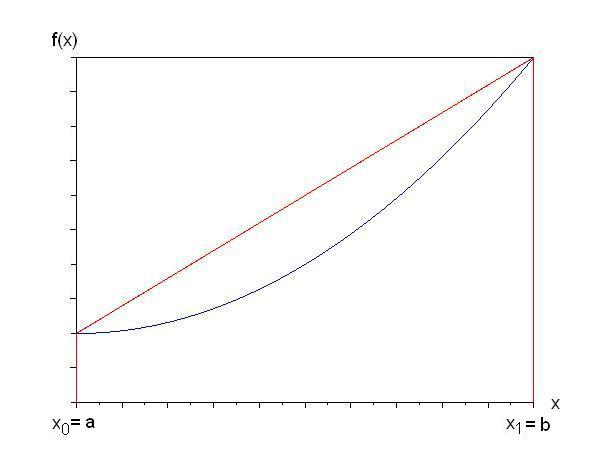
\includegraphics[scale=0.7]{./cap_integracao/pics/int_2/int_2}
% \end{center}

Desta forma, utilizando $x_1:=a$,  $x_2:=b$, $h=x_2-x_1$ e a notação $f_i=f(x_i)$ obtemos através da interpolação de Lagrange o polinômio
\begin{eqnarray} 
p_1(x) &=& f_1 L_1(x)+ f_2 L_2(x) 
\end{eqnarray}
Aproximando $f(x)$ por $p_1(x)$ e integrando obtemos
\begin{eqnarray*}
  \int_a^bf(x)\;dx &\approx& \int_a^bp_1(x)\;dx \\
    &=& \int_a^b f_1L_1(x) + f_2L_2(x)\;dx \\
    &=& f_1 \int_a^b L_1(x)\;dx + f_2 \int_a^b L_2(x)\;dx \\
    &=& A_1 f_1 + A_2 f_2 
\end{eqnarray*}
onde
\begin{eqnarray*}
  A_1 &=& \int_a^b\frac{x-x_1}{x_2-x_1}dx =  \left[\frac{(x-x_1)^2}{2h}\right]_{x_1}^{x_2}\\
      &=& \frac{(x_2-x_1)^2}{2h} = \frac{h^2}{2h} = \frac{1}{2}h
\end{eqnarray*}
Da mesma forma,
\begin{eqnarray*}
  A_2 &=& \int_a^b\frac{(x-x_2)}{(x_1-x_2)}dx = \frac{1}{2}h
\end{eqnarray*}


de onde obtemos a \emph{regra do trapézio} dada por
\begin{equation}
  \int_a^b f(x)\;dx \approx \left(\frac{1}{2}f_1 + \frac{1}{2}f_2\right)h 
\end{equation}


\subsubsection{Erro na regra do trapézio}
O \textit{erro na regra do trapézio} pode ser obtida integrando o erro da interpolação de Lagrange,
\begin{eqnarray*}
   E_{TRAP} = \int_a^b E^2_{LAG}(x) \;dx= \int_a^b \frac{f''(\xi(x))}{2!}(x-x_1)(x-x_2) \;dx
\end{eqnarray*}
Pelo teorema do valor médio, existe $a\leq \eta\leq b$ tal que
\begin{eqnarray*}
    E_{TRAP} = \frac{f''(\eta)}{2!}\int_a^b (x-x_1)(x-x_2) \;dx,
\end{eqnarray*}
portanto
\begin{eqnarray*}
     E_{TRAP}
  &=& \frac{f''(\eta)}{2}\left[\frac{x^3}{3}-\frac{x^2}{2}(x_2+x_1)+x_1x_2x\right]_{x_1}^{x_2}\\
  &=& \frac{f''(\eta)}{2}\left(\frac{x_2^3}{3}-\frac{x_2^2}{2}(x_2+x_1)+x_1x_2x_2-\frac{x_1^3}{3}+\frac{x_1^2}{2}(x_2+x_1)-x_1x_2x_1\right)\\
  &=& \frac{f''(\eta)}{2}\frac{2x_2^3-3x_2^2(x_2+x_1)+6x_2^2x_1-2x_1^3+3x_1^2(x_2+x_1)-6x_2x_1^2}{6}\\
  &=& \frac{f''(\eta)}{12}\left(x_1^3-3x_1^2x_2+3x_2^2x_1-x_2^3\right) 
   =  \frac{f''(\eta)}{12}(x_1-x_2)^3\\
  &=& -\frac{f''(\eta)}{12}h^3.
\end{eqnarray*}

Assim o erro na regra do trapézio é 
$$
E_{TRAP}  = -\frac{f''(\eta)}{12}h^3 = \mathcal{O}(h^3).
$$

\begin{ex}
Use a regra do trapézio para aproximar a integral
$$
\int_0^1e^{-x^2}dx.
$$
Depois divida a integral em duas
$$
\int_0^{1/2}e^{-x^2}dx+\int_{1/2}^{1}e^{-x^2}dx.
$$
e aplique a regra do trapézio em cada uma delas. Finalmente, repita o processo dividindo em quatro integrais.
\end{ex}
Usando o intervalo $[0,1]$, temos $h=1$, $x_0=0$ e $x_1=1$. A regra do trapézio resulta em
$$
\int_0^1e^{-x^2}dx\approx \frac{1}{2}(e^{0}+e^{-1})=0,6839397
$$
Usando dois intervalos, $[0,1/2]$ e $[1/2,1]$ e usando a regra do trapézio em cada um dos intervalos, temos:
\begin{eqnarray*}
\int_0^1e^{-x^2}dx &\approx& \frac{0,5}{2}\left(e^{0}+e^{-1/4}\right) + \frac{0,5}{2}\left(e^{-1/4}+e^{-1}\right) \\
&=& 0,4447002+0,2866701 =0,7313703.
\end{eqnarray*}
Agora, usando quatro intervalos, temos
\begin{eqnarray*}
\int_0^1e^{-x^2}dx &\approx& \frac{0,25}{2}\left(e^{0}+e^{-1/16}\right) + \frac{0,25}{2}\left(e^{-1/16}+e^{-1/4}\right) \\
&+& \frac{0,25}{2}\left(e^{-1/4}+e^{-9/16}\right)+\frac{0,25}{2}\left(e^{-9/16}+e^{-1}\right) \\
&=& 0,7429841
\end{eqnarray*}



\subsection{Regra de Simpson}\index{integração numérica!regra de Simpson}
Na regra de Simpson aproximamos $f$ por um polinômio de grau $2$, portanto precisamos três pontos do intervalo $[a,b]$. Utilizando, por definição,
$$
x_1:=a,\qquad x_2:=\frac{a+b}{2}\qquad \text{e}\qquad x_3:=b
$$
com $h=x_3-x_1$, podemos obter o polinômio de Lagrange 
\begin{equation*}
    p_2(x) = f_1L_1(x) + f_2L_2(x)  + f_3L_3(x)
\end{equation*}

Aproximando $f$ por $p_2$ e integrando temos
\begin{eqnarray}
\int_a^bf(x)dx &\approx&\int_a^b p_2(x) \;dx \\ 
               &=&\int_a^b f_1L_1(x) + f_2L_2(x)  + f_3L_3(x) \;dx \\  
               &=&f_1 A_1 + f_2A_2  + f_3A_3  
\end{eqnarray}
onde
\begin{eqnarray}
  A_i = \int_a^b L_i(x) \;dx  
\end{eqnarray}
Calculando essas integrais obtemos \emph{a regra de Simpson}
$$
\int_a^bf(x)dx=\left(\frac{1}{6}f(x_1)+\frac{4}{6}f(x_2)+\frac{1}{6}f(x_3)\right)h.
$$

\begin{ex}
Obtenha os coeficientes $A_i$ do método de Simpson  integrando os polinômios de Lagrange $L_i(x)$.

Fazendo uma translação para a origem (subtraindo $x_1$ de $x_2$ e $x_3$)
\begin{eqnarray*}
   A_1 &=& \int_{x_1}^{x_3} \frac{(x-x_2)(x-x_3)}{(x_1-x_2)(x_1-x_3)}\;dx \\
       &=& \int_0^h \frac{(x-h/2)(x-h)}{(0-h/2)(0-h)}\;dx 
        =  \frac{2}{h^2} \int_0^h (x-h/2)(x-h)\;dx \\
       &=& \frac{2}{h^2} \int_0^h x^2 -\frac{3}{2}hx+\frac{h^2}{2}\;dx 
        =  \frac{2}{h^2} (x^3/3 -\frac{3}{4}hx^2+\frac{h^2x}{2})_0^h \\  
       &=& \frac{2}{h^2} (h^3/3 -\frac{3}{4}h^3+\frac{h^3}{2})   
        =  (\frac{2}{3}-\frac{3}{2}+1)h\\
       &=& \frac{1}{6}h
\end{eqnarray*}
Apesar de longa, é apenas a integral de um polinômio de grau 2. De forma semelhante podemos obter
$$
A_2 = \frac{4}{6}h, \;\;\; A_3 = \frac{1}{6}h
$$
\end{ex}



\subsubsection{Erro na regra de Simpson}\index{integração numérica!regra de Simpson}
Se usarmos a mesma metodologia da regra dos trapézios, teremos
$$
\int_a^bf(x)dx=\int_a^bp_2(x)dx+\int_a^b\frac{(x-x_1)(x-x_2)(x-x_3)}{6}f'''(\xi(x))dx
$$
e obteremos o fórmula de Simpson com um erro de quarta ordem. O fato é que a regra de Simpson tem ordem cinco e, para isso, usaremos uma abordagem alternativa.

Considere o polinômio de Taylor em $x_2$,
$$
f(x)=f(x_2)+f'(x_2)(x-x_2)+\frac{f''(x_2)}{2}(x-x_2)^2+\frac{f'''(x_2)}{6}(x-x_2)^3+\frac{f^{(4)}(\xi(x))}{24}(x-x_2)^4,
$$
onde $x_1\leq\xi(x)\leq x_3$ e integre no intervalo $[a,b]=[x_1,x_3]$:
\begin{equation*}
  \begin{split}
    \int_a^bf(x)dx&= \left[f(x_2)(x-x_2)+f'(x_2)\frac{(x-x_2)^2}{2} + \frac{f''(x_2)}{6}(x-x_2)^3\right. \\
      &\left. + \frac{f'''(x_2)}{24}(x-x_2)^4\right]_{x_1}^{x_3}\\
      &+ \frac{1}{24}\int_{x_1}^{x_3}f^{(4)}(\xi(x))(x-x_2)^4dx,    
  \end{split}
\end{equation*}
Pelo teorema do valor médio, existe $x_1\leq\eta\leq x_3$ tal que
\begin{equation*}
  \begin{split}
    \int_a^bf(x)dx&= \left[f(x_2)(x-x_2)+f'(x_2)\frac{(x-x_2)^2}{2}+\frac{f''(x_2)}{6}(x-x_2)^3\right.\\
    &+\left.\frac{f'''(x_2)}{24}(x-x_2)^4\right]_{x_1}^{x_3}\\
    &+ \frac{f^{(4)}(\eta)}{24}\int_{x_1}^{x_3}(x-x_2)^4dx\\
    &= \left[f(x_2)(x-x_2)+f'(x_2)\frac{(x-x_2)^2}{2}+\frac{f''(x_2)}{6}(x-x_2)^3\right.\\
    &+\left.\frac{f'''(x_2)}{24}(x-x_2)^4\right]_{x_1}^{x_3}\\
    &+ \frac{f^{(4)}(\eta)}{120}\left[(x-x_2)^5\right]_{x_1}^{x_3}    
  \end{split}
\end{equation*}
Usando o fato que
$$
(x_3-x_2)^3-(x_1-x_2)^3=2h^3,
$$
$$
(x_3-x_2)^4-(x_1-x_2)^4=0
$$
e
$$
(x_3-x_2)^5-(x_1-x_2)^5=2h^5,
$$
temos
$$
\int_a^bf(x)dx=hf(x_2)+\frac{h^3}{3}f''(x_2)+\frac{h^5f^{(4)}(\eta)}{60}.
$$
Usando a fórmula de diferenças finitas centrais para a derivada segunda:
$$
f''(x_2)=\frac{f(x_1)-2f(x_2)+f(x_3)}{h^2}+\frac{h^2}{12}f^{(4)}(\eta_2),
$$
$x_1\leq \eta_2\leq x_3$, temos
\begin{eqnarray*}
\int_a^bf(x)dx&=&2hf(x_2)+\frac{h^3}{3}\left(\frac{f(x_1)-2f(x_2)+f(x_3)}{h^2}+\frac{h^2}{12}f^{(4)}(\eta_2)\right)\\
&+&\frac{h^5f^{(4)}(\eta)}{60}\\
&=&\frac{h}{3}\left(f(x_1)+4f(x_2)+f(x_3)\right)-\frac{h^5}{12}\left(\frac{1}{3}f^{(4)}(\eta_2)-\frac{1}{5}f^{(4)}(\eta)\right).
\end{eqnarray*}
Pode-se mostrar que é possível escolher $\eta_3$ que substitua $\eta$ e $\eta_2$ com a seguinte estimativa
$$
\int_a^bf(x)dx=\frac{h}{3}\left(f(x_1)+4f(x_2)+f(x_3)\right)-\frac{h^5}{90}f^{(4)}(\eta_3).
$$

\begin{ex}
Use a regra de Simpson para aproximar a integral
$$
\int_0^1e^{-x^2}dx.
$$
Depois divida a integral em duas
$$
\int_0^{1/2}e^{-x^2}dx+\int_{1/2}^{1}e^{-x^2}dx.
$$
e aplica a regra de Simpson em cada uma delas.
\end{ex}
Usando o intervalo $[0,1]$, temos $h=1/2$, $x_0=0$, $x_1=1/2$ e $x_2=1$. A regra de Simpson resulta em
$$
\int_0^1e^{-x^2}dx\approx \frac{0,5}{3}(e^{0}+4e^{-1/4}+e^{-1})=0,7471804
$$
Usando dois intervalos, $[0,1/2]$ e $[1/2,1]$ e usando a regra do trapézio em cada um dos intervalos, temos:
$$
\int_0^1e^{-x^2}dx\approx \frac{0,25}{3}(e^{0}+4e^{-1/16}+e^{-1/4})+\frac{0,25}{3}(e^{-1/4}+4e^{-9/16}+e^{-1})=0,7468554
$$

\subsection*{Exercícios}

\begin{exer}Calcule numericamente as seguintes integrais:
  \begin{eqnarray*}
    \text{a)}~\int_0^1e^{-x}\,dx & \text{b)}~\int_0^1x^2\,dx\\
    \text{c)}~\int_0^1x^3\,dx & \text{d)}~\int_0^1xe^{-x^2}\,dx\\
    \text{e)}~\int_0^1\frac{1}{x^2+1}\,dx &\text{e)}~\int_0^1\frac{x}{x^2+1}dx 
  \end{eqnarray*}
usando os métodos simples do Ponto médio, Trapézio e Simpson. Calcule, também, o valor analítico destas integrais e o erro nas aproximações dadas pelas quadraturas numérica.
\end{exer}
% \begin{resp}
%   
%  \begin{center}
% \begin{tabular}{|c|c|c|c|c|}
% \hline
%   & exato & Ponto médio & Trapézio & Simpson \\
% \hline
%  & & & &\\[-.3cm]
% $\int_0^1e^{-x}dx$ &$1-e^{-1}\approx 0.6321206$& $ e^{-1/2}\approx 0.6065307$&$\frac{1+e^{-1}}{2}\approx 0.6839397$ &$\frac{1+4e^{-1/2}+e^{-1}}{6}\approx 0.6323337$\\[.2cm]
% \hline
%  & & & &\\[-.3cm]
% $\int_0^1x^2dx $ & $1/3\approx 0.3333333$& 0.25 & 0.5 & 0.3333333\\[.2cm]

% \hline
%  & & & &\\[-.3cm]
% $\int_0^1x^3dx $ & $1/4=0.25$ & 0.125 & 0.5 & 0.25\\[.2cm]
% \hline
%  & & & &\\[-.3cm]
% $\int_0^1xe^{-x^2}dx$  &$\frac{1}{2}\left(1-e^{-1}\right)\approx 0.3160603$ & 0.3894004  &  0.1839397 &   0.3209135  \\[.2cm]
% \hline
%  & & & &\\[-.3cm]
% $\int_0^1\frac{1}{x^2+1}dx$  & $\tan^{-1}(1)\approx 0.7853982$ &  0.8  &  0.75 &   0.7833333  
%  \\[.2cm]
% \hline
%  & & & &\\[-.3cm]
% $\int_0^1\frac{x}{x^2+1}dx$  &$\frac{1}{2}\ln(2)\approx  0.3465736  $ & 0.4 & 0.25 & 0.35\\[.2cm]
% \hline
%  & & & &\\[-.3cm]
% $\int_0^1\frac{1}{x+1}dx$  & $\ln(2) \approx 0.6931472$ & 0.6666667  &  0.75 &   0.6944444  \\[.2cm]
% \hline
% \end{tabular}
% \end{center}    
%   
% \end{resp}

\begin{exer}
 Dê a interpretação geométrica dos métodos do ponto médio, trapézio e Simpson. A partir desta construção geométrica, deduza as fórmulas para aproximar 
 $$\int_a^bf(x)dx.$$
 Verifique o método de Simpson pode ser entendido como uma média aritmética ponderada entre os métodos de trapézio e ponto médio. Encontre os pesos envolvidos. Explique o que são os métodos compostos.
 \end{exer}
\begin{resp}
  
$$ I_{Simpson}= \frac{1}{3} I_{Trap}+ \frac{2}{3}I_{PM}$$    
  
\end{resp}


\begin{exer}
Calcule numericamente o valor de $\int_2^5e^{4-x^2}dx$ usando os métodos compostos do ponto médio, trapézio e Simpson. Obtenha os resultados utilizando, em cada quadratura, o número de pontos indicado.
\begin{center}
\begin{tabular}{|c|c|c|c|c|}
\hline
n   & Ponto médio & Trapézios & Simpson \\
\hline
$3$ &~\hspace{40pt}~& ~\hspace{40pt}~& ~\hspace{40pt}\\
\hline
$5 $ & & & \\
\hline
$7 $ & & &\\
\hline
$9$  & & &\\
\hline
\end{tabular}
\end{center}
\end{exer}
\begin{resp}
  
    \begin{equation*}
    \begin{array}{c|cccc}
        n   & \text{Ponto médio} & \text{Trapézios} & \text{Simpson} \\  \hline
        3 & 0.1056606  &  0.7503919  &  0.5005225  \\  \hline
        5 & 0.1726140 &   0.3964724  &  0.2784992   \\\hline
        7 & 0.1973663 &   0.3062023  &  0.2393551  \\ \hline
        9  &  0.2084204 &   0.2721145  &  0.2306618  \\ \hline
        \multicolumn{5}{c}{}      
    \end{array}      
    \end{equation*}
  
\end{resp}



\section{Obtenção das regras de quadratura}

Na seção anterior, obtivemos as regras de quadraturas pela aproximação do integrando por polinômios interpoladores de Lagrange. Aqui, veremos um outro método para obter regras de quadratura, que torna-se bastante útil para quando temos muitos pontos ou quando o intervalo entre os pontos não é uniforme.

Dados $n$ pontos $[t_1,t_2,\ldots ,t_n]$, queremos obter uma aproximação para
\begin{align}\label{regraint}
  \int _a^b f(t) \;dt \approx w_1f(t_1)+w_2f(t_2)+\ldots +w_nf(t_n)
\end{align}
que seja exata para polinômios\footnote{Por exemplo, se $n=2$, então a regra é exata para retas.} até ordem  $n-1$.

Aproxime $f(t)$ pelo polinômio $p(t)=w_1\phi_1(t)+\ldots +w_n \phi_n(t)$ de ordem $n-1$. Escolha uma base, como por exemplo $\phi _k(t)=t^{k-1}$. Como a regra de quadratura deve ser exata para qualquer polinômio até ordem $n-1$, então também deve ser exata para qualquer função da base. Substituindo $f(t)$ por $\phi _1(t)=1$ em \eqref{regraint} obtemos 
\begin{eqnarray}
\int _a^b \phi_1(t) \; dt = t|_a^b &=&  w_1\phi _1(t_1)+w_2\phi _1(t_2)+\ldots +w_n\phi_1(t_n) \\
                              b-a  &=&  w_1+w_2+\ldots +w_n
\end{eqnarray}

Da mesma forma para $\phi_k(t)$, $k=2,\ldots,n$, obtemos
\begin{align}
   (t^2/2)|_a^b = \frac{b^2-a^2}{2} &=  w_1t_1  +w_2t_2  +\ldots +w_nt_n   \\
   (t^3/3)|_a^b = \frac{b^3-a^3}{3} &=  w_1t_1^2+w_2t_2^2+\ldots +w_nt_n^2 \\
                    \vdots          &=  \vdots    \\
 \frac{b^{n}-a^{n}}{n}              &=  w_1t_1^{n-1}+w_2t_2^{n-1}+\ldots +w_nt_n^{n-1}
\end{align}
que pode ser escrito na forma matricial
\begin{equation}
\begin{bmatrix}
    1     &  1    & \ldots   &  1 \\
    t_1   &  t_2   & \ldots   & t_n \\
    t_1^2 &  t_2^2  & \ldots   & t_n^2 \\
    \vdots    &  \vdots     &    & \vdots   \\
    t_1^{n-1} & t_2^{n-1} & \ldots   & t_n^{n-1}
\end{bmatrix}
\begin{bmatrix}  w_1 \\ w_2\\ w_3  \\ \vdots   \\ w_n     \end{bmatrix}
=
\begin{bmatrix}  b-a  \\ \frac{b^2-a^2}{2} \\ \frac{b^3-a^3}{3} \\ \vdots  \\ \frac{b^{n}-a^{n}}{n}  \end{bmatrix}
\end{equation}
Resolvendo o sistema obtemos os coeficientes $w_k$ para a regra de integração.

\begin{ex}
Seja $n=3$, $[a,b]=[0,h]$, onde $[t_1,t_2,t_3]=[0,h/2,h]$. Obtenha uma regra de integração para aproximar $\int _a^b f(t)\;dt$.
\end{ex}
\begin{sol}
A regra terá a forma
\begin{align}
  \int _a^b f(t)\;dt & \approx w_1f(t_1)+w_2f(t_2)+w_3f(t_3)\\
                 & \approx w_1f_1   +w_2f_2   +w_3f_3
\end{align}
Considere a base polinomial $[\phi _1(t),\phi _2(t),\phi _3(t)]=[1,t,t^2]$ e substitua $f(t)$ por $\phi_k(t)$ obtendo
\begin{align}
   \int _0^h 1   \;dt = h     &=  w_1(1)   +w_2(1)     + w_3(1) \\
   \int _0^h t   \;dt = h^2/2 &=  w_1(0)   +w_2(h/2)   + w_3(h) \\
   \int _0^h t^2 \;dt = h^3/3 &=  w_1(0)^2 +w_2(h/2)^2 + w_3(h)^2
\end{align}
que pode ser escrito na forma matricial
\begin{equation}
\begin{bmatrix}
    1  &  1    &  1 \\
    0  &  h/2    & h  \\
    0  &  h^2/4    & h^2
\end{bmatrix}
\begin{bmatrix}
 w_1 \\ w_2\\ w_3
\end{bmatrix}
=
\begin{bmatrix}
 h  \\ h^2/2 \\ h^3/3
\end{bmatrix}
\end{equation}
Note que podemos simplificar $h$ tal que o sistema fique
\begin{equation}
\begin{bmatrix}
    1  &  1    &  1 \\
    0  &  1/2  & 1  \\
    0  &  1/4  & 1
\end{bmatrix}
\begin{bmatrix}
 w_1 \\ w_2\\ w_3
\end{bmatrix}
=
h
\begin{bmatrix}
 1  \\ 1/2 \\ 1/3
\end{bmatrix}
\end{equation}

Resolvendo o sistema obtemos $\displaystyle [w_1,w_2,w_3]=h[\frac{1}{6},\frac{4}{6},\frac{1}{6}]$ fornecendo a regra de Simpson
\begin{equation}
  \int _0^h f(t) \;dt \approx  \frac{h}{6}f_0+\frac{4h}{6}f_1+\frac{h}{6}f_2
\end{equation}
\end{sol}

>>>>>>> 070aee735edae39b9603913dda7d0ba033e9e218








\section{Regras compostas}\index{integração numérica!regras compostas}

Vimos que em todas as estimativas de erro que derivamos, o erro depende do tamanho do intervalo de integração. Uma estratégia para reduzir o erro consiste em particionar o intervalo de integração em diversos subintervalos menores tal que
\begin{equation*}
\int_{a}^b f(x)dx=\sum_{i=1}^{n} \int_{x_i}^{x_{i+1}} f(x)\;dx 
\end{equation*}
onde $a=x_1<...<x_{n+1}=b$, sendo $n$ o número de subintervalos da partição do intervalo de integração. No caso uniforme $x_i = a + (i-1)h$, $h = (b-a)/n$.

Depois, aplica-se um método simples de integração em cada subintervalo,
$$
\int_{x_i}^{x_{i+1}} f(x)\;dx \approx \Delta S_i
$$
e a integral será aproximada por
$$
\int_a^b f(x)\;dx \approx S= \sum_{i=1}^{n} \Delta S_i
$$

%%%%%%%%%%%%%%%%%%%%
% scilab
%%%%%%%%%%%%%%%%%%%%
\ifisscilab
\subsection{Código Scilab: Regras compostas em geral}
Devemos fazer um loop sobre todos os intervalos e para cada intervalo aplicamos uma regra de quadratura. 

\verbatiminput{./cap_integracao/codes/simpson.sci}

Acumulamos o valor da integral em \verb+S+. No código acima temos o método de Simpson, mas basta trocarmos a fórmula para termos outras quadraturas.

Note que esta não é a implementação mais eficiente, pois reutiliza os termos no contorno dos intervalos. Nas próximas seções veremos regras compostas específicas para alguns métodos.
\fi
%%%%%%%%%%%%%%%%%%%%

\subsection{Método composto dos trapézios}\index{integração numérica!método composto!dos trapézios}
A \emph{regra composta dos trapézios} assume a seguinte forma:
\begin{eqnarray*}
  \int_{a}^b f(x)dx &=& \sum_{i=1}^{n} \int_{x_i}^{x_{i+1}}f(x)\,dx \\
  &\approx& \sum_{i=1}^{n} \frac{x_{i+1}-x_i}{2}\left[f(x_i)+f(x_{i+1})\right]
\end{eqnarray*}
Como $h = x_{i+1} - x_i$, temos:
\begin{eqnarray*}
\int_{a}^b f(x)\,dx &\approx& \frac{h}{2}\sum_{k=1}^{N_i}\left[f(x_k)+f(x_{k+1})\right]\\
&=& \frac{h}{2}\left[f(x_1)+2f(x_2)+2f(x_3)+\cdots + 2f(x_{N_i})+f(x_{N_i+1})\right]\\
&=& \frac{h}{2}\left[f(x_1) + f(x_{N_i+1})\right] + h\sum_{i=2}^{N_i} f(x_i)
\end{eqnarray*}

\ifisscilab

\subsection{Código Scilab: trapézio composto}
O código Scilab abaixo é uma implementação do método do trapézio composto para calcular:
\begin{equation*}
  \int_a^b f(x)\,dx = \frac{h}{2}\left[f(x_1) + f(x_{n+1})\right] + h\sum_{i=2}^n f(x_i) + O(h^3),
\end{equation*}
onde $h = (b-a)/n$ e $x_i = a + (i-1)h$, $i=1,2,\dotsc,n+1$. Os parâmetros de entrada são: \verb+f+ o integrando definido como uma função no Scilab, \verb+a+ o limite inferior de integração, \verb+b+ o limite superior de integração, \verb+n+ o número de subintervalos desejado. A variável de saída é \verb+y+ e corresponde a aproximação calculada de $\int_a^b f(x)\, dx$.

\verbatiminput{./cap_integracao/codes/trap_comp/trap_comp.sci}
\fi

\subsection{Método composto de Simpson}\index{integração numérica!método composto!de Simpson}
Já a regra composta de Simpson assume a seguinte forma:
\begin{eqnarray*}
  \int_{a}^b f(x)\,dx &=& \sum_{k=1}^{n} \int_{x_k}^{x_{k+1}} f(x)dx \\
  &\approx& \sum_{k=1}^{n} \frac{x_{x+1}-x_k}{6}\left[f(x_k) + 4f\left(\frac{x_{k+1}+x_k}{2}\right)+f(x_{k+1})\right]
\end{eqnarray*}
onde, como anteriormente, $x_k = a + (k-1)h$, $h = (b-a)/n$ e $i = 1,2,\dotsc,n+1$, sendo $n$ o número de subintervalos da partição do intervalo de integração. Podemos simplificar o somatório acima, escrevendo:
\begin{equation*}
  \int_{a}^b f(x)\,dx \approx \frac{h}{3}\left[f(x_1) + 2\sum_{i=1}^{n-1} f(x_{2i+1}) + 4\sum_{i=1}^{n} f(x_{2i}) + f(x_{2n+1})\right] + O(h^5)
\end{equation*}
onde, agora, $h = (b-a)/(2n)$, $x_i = a + (i-1)h$, $i=1,2,\dotsc,2n+1$.

\ifisscilab
\subsection{Código Scilab: Simpson composto}
O código Scilab abaixo é uma implementação do método de Simpson composto para calcular:
\begin{equation*}
  \int_a^b f(x)\,dx = \frac{h}{3}\left[f(x_1) + 2\sum_{i=1}^{n-1} f(x_{2i+1}) + 4\sum_{i=1}^{n} f(x_{2i}) + f(x_{2n+1})\right] + O(h^3),
\end{equation*}
onde $h = (b-a)/(2n)$ e $x_i = a + (i-1)h$, $i=1,2,\dotsc,2n+1$. Os parâmetros de entrada são: \verb+f+ o integrando definido como uma função no Scilab, \verb+a+ o limite inferior de integração, \verb+b+ o limite superior de integração, \verb+n+ o número de subintervalos desejado. A variável de saída é \verb+y+ e corresponde a aproximação calculada de $\int_a^b f(x)\, dx$.
\verbatiminput{./rotinas/Derivacao_e_integracao/simp_comp.sci}
\fi

\begin{ex}Calcule numericamente a integral
$$
\int_0^2 x^2 e^{x^2}dx
$$
pelas regras compostas do ponto médio, trapézio e Simpson variando o número de intervalos \\$N_i=1,\ 2,\ 3,\ 6,\ 12,\ 24,\ 48,\ 96$.
\end{ex}
\begin{sol}
  \begin{equation*}
  \begin{array}{c|ccc}\hline
    n &  \text{Ponto Médio} &  \text{Trapézios} & \text{Simpson}\\ \hline
    1 & 5,4365637&218,3926&76,421909\\
    2&21,668412&111,91458&51,750469\\
    3&31,678746&80,272022&47,876505\\
    6&41,755985&55,975384&46,495785\\
    12&45,137529&48,865685&46,380248\\
    24&46,057757&47,001607&46,372373\\
    48&46,292964&46,529682&46,37187\\
    96&46,352096&46,411323&46,371838\\\hline
    \multicolumn{4}{c}{}
  \end{array}    
  \end{equation*}
\end{sol}

\subsection*{Exercícios}

\begin{exer}
Use as rotinas construídas em aula e calcule numericamente o valor das seguintes integrais usando o método composto dos trapézios para os seguintes números de pontos:
$$
\begin{array}{|c|c|c|c|c|c|}
\hline
n   &h& \int_{0}^1e^{-4x^2}dx & \int_{0}^1\frac{1}{1+x^2}dx & \int_{0}^1x^4(1-x)^4dx & \int_{0}^1e^{-\frac{1}{x^2+1}}dx  \\
\hline
$17$ && 0.4409931& & ~\hspace{40pt}~& ~\hspace{40pt}~\\
\hline
$33 $ &&0.4410288    &      & & \\
\hline
$65 $  &&0.4410377  &   & &\\
\hline
$129$   &&0.4410400 &  & &\\
\hline
$257$   &&0.4410405 &  & &\\
\hline
$513$   &&0.4410406 & & &\\
\hline
$1025$   &&0.4410407&0.7853981 &1.5873015873016\cdot 10^{-3} &4.6191723776309\cdot 10^{-1} \\
\hline
\end{array}
$$
\end{exer}


\begin{exer}
O valor exato da integral imprópria $\int_0^1x\ln(x)dx$ é dado por
$$\int_0^1x\ln(x)dx=\left.\left(\frac{x^2}{2}\ln x-\frac{x^2}{4}\right)\right|_0^1=-1/4$$
Aproxime o valor desta integral usando a regra  de Simpson para $n=3$, $n=5$ e $n=7$. Como você avalia a qualidade do resultado obtido? Por que isso acontece.
\end{exer}
\begin{resp}
  
-0.2310491, -0.2452073, - 0.2478649.    
  
\end{resp}

\begin{exer}
O valor exato da integral imprópria $\int_0^\infty e^{-x^2}dx$ é dado por $\frac{\sqrt{\pi}}{2}$.
Escreva esta integral como
$$I=\int_0^1 e^{-x^2}dx+\int_0^1 u^{-2} e^{-1/u^2}du=\int_0^1 \left(e^{-x^2}+x^{-2}e^{-1/x^2}\right)dx$$
e aproxime seu valor usando o esquema de trapézios e Simpson para $n=5$, $n=7$ e $n=9$.
\end{exer}

\begin{exer}
Estamos interessados em avaliar numericamente a seguinte integral:
$$\int_0^1 \ln(x)\sin(x)dx$$
cujo valor com 10 casas decimais corretas é $-.2398117420$.
\begin{itemize}
\item[a)] Aproxime esta integral via Gauss-Legendre com $n=2$,$n=3$, $n=4$, $n=5$, $n=6$ e $n=7$.
\item[b)] Use a identidade
\begin{eqnarray*}
\int_0^1 \ln(x)\sin(x)dx&=&\int_0^1 \ln(x)xdx+\int_0^1 \ln(x)\left[\sin(x)-x\right]dx\\
&=&\left.\left(\frac{x^2}{2}\ln x-\frac{x^2}{4}\right)\right|_0^1+\int_0^1 \ln(x)\left[\sin(x)-x\right]dx\\
&=&-\frac{1}{4}+\int_0^1 \ln(x)\left[\sin(x)-x\right]dx
\end{eqnarray*}
e aproxime a integral $\int_0^1 \ln(x)\left[\sin(x)-x\right]dx$ numericamente via Gauss-Legendre com $n=2$, $n=3$, $n=4$, $n=5$, $n=6$ e $n=7$.
\item[c)] Compare os resultados e discuta levando em consideração as respostas às seguintes perguntas: 1)Qual função é mais bem-comportada na origem? 2)Na segunda formulação, qual porção da solução foi obtida analiticamente e, portanto, sem erro de truncamento?
\end{itemize}
\end{exer}
\begin{resp}
  
    a)-0.2472261,  -0.2416451,  -0.2404596,  -0.2400968,  -0.2399563,  -0.2398928.
    b)-0.2393727,  -0.2397994,  -0.2398104,  -0.2398115,  -0.2398117,  -0.2398117.  
  
\end{resp}

\section{O método de Romberg}\index{integração numérica!método de Romberg}
O método de Romberg é um método simplificado para construir quadraturas de alta ordem.

Considere o método de trapézios composto aplicado à integral
$$\int_a^bf(x)dx$$
Defina $I(h)$ a aproximação desta integral pelo método dos trapézios composto com  malha de largura constante igual a h. Aqui $h=\frac{b-a}{N_i}$ para algum $N_i$ inteiro, i.e.:
$$I(h)=\frac{h}{2}\left[f(a)+2\sum_{j=2}^{N_i} f(x_j)+ f(b)\right],~~~N_i=\frac{b-a}{h}$$

\begin{teo} Se $f(x)$ é uma função analítica no intervalo $(a,b)$, então a função $I(h)$ admite uma representação na forma
$$I(h)=I_0 + I_2 h^2 + I_4{h^4}+ I_6{h^6}+\ldots$$
\end{teo}
Para um demonstração, veja \cite{DEMAILLY}. Em especial observamos que
$$\int_a^b f(x)dx = \lim_{h\to 0}I(h)=I_0$$
Ou seja, o valor exato da integral procurada é dado pelo coeficiente $I_0$.

A ideia central do método de Romberg, agora, consiste em usar a extrapolação de Richardson para construir métodos de maior ordem a partir do métodos dos trapézios para o intervalo $(a,b)$
\begin{ex} \label{exemplo_romberg_1}Construção do método de quarta ordem.
\begin{eqnarray*}
I(h)&=&I_0 + I_2 h^2 + I_4{h^4}+ I_6{h^6}+\ldots\\~\\
I\left(\frac{h}{2}\right)&=&I_0 + I_2 \frac{h^2}{4} + I_4\frac{h^4}{16}+ I_6\frac{h^6}{64}+\ldots\\
\end{eqnarray*}
Usamos agora uma eliminação gaussiana para obter o termo $I_0$:
\begin{eqnarray*}
\frac{4I(h/2)-I(h)}{3}=I_0-\frac{1}{4}I_4h^4-\frac{5}{16}I_6h^6+\ldots
\end{eqnarray*}
Vamos agora aplicar a fórmula para $h=b-a$,
\begin{eqnarray*}
I(h)&=& \frac{h}{2} \left[f(a)+f(b)\right]\\
I(h/2)&=& \frac{h}{4} \left[f(a)+2f\left(c\right)+f(b)\right],~~ c=\frac{a+b}{2}\\
\end{eqnarray*}

\begin{eqnarray*}
\frac{4I(h/2)-I(h)}{3}&=&\frac{h}{3}\left[f(a)+2f\left(c\right)+f(b)\right]-\frac{h}{6} \left[f(a)+f(b)\right]\\
&=&\frac{h}{6}\left[f(a)+4f\left(c\right)+f(b)\right]
\end{eqnarray*}
Observe que esquema coincide com o método de Simpson.
\end{ex}

A partir de agora, usaremos a seguinte notação
\begin{eqnarray*}
R_{1,1}&=&I(h)\\
R_{2,1}&=&I(h/2)\\
R_{3,1}&=&I(h/4)\\
&\vdots&\\
R_{n,1}&=&I(h/2^{n-1})
\end{eqnarray*}

Observamos que os pontos envolvidos na quadratura $R_{k,1}$ são os mesmos pontos envolvidos na quadratura $R(k-1,1)$ acrescidos dos pontos centrais, assim, temos a seguinte fórmula de recorrência:
$$R_{k,1}=\frac{1}{2}R_{k-1,1}+\frac{h}{2^{k-1}} \sum_{i=1}^{2^{k-2}}f\left(a+(2i-1)\frac{h}{2^{k-1}}\right)$$

Definimos $R_{k,2}$ para $k\geq 2$ como o esquema de ordem quatro obtido da fórmula do exemplo \ref{exemplo_romberg_1}:
$$R_{k,2}=\frac{4R_{k,1}-R_{k-1,1}}{3}$$
Os valores $R_{k,2}$ representam então os valores obtidos pelo método de Simpson composto aplicado a uma malha composta de $2^{k-1}+1$ pontos.

Similarmente os valores de $R_{k,j}$ são os valores obtidos pela quadratura de ordem $2j$ obtida via extrapolação de Richardson. Pode-se mostrar que
$$R_{k,j}=R_{k,j-1}+\frac{R_{k,j-1}-R_{k-1,j-1}}{4^{j-1}-1}.$$

\begin{ex} 
Construa o esquema de Romberg para aproximar o valor de $\int_0^2e^{-x^2}dx$ com erro de ordem 8.

O que nos fornece os seguintes resultados:
\begin{tabular}{|c|c|c|c|}\hline
    55,59815  &   0,000000    &       0,000000  &         0,000000         \\
    30,517357 &   22,157092 &   0,000000   &        0,000000         \\
    20,644559 &   17,353626 &   17,033395 &   0,000000         \\
    17,565086 &   16,538595  &  16,484259 &   \pmb{16,475543}  \\\hline
\end{tabular}

Ou seja, temos:
\begin{equation*}
  \int_0^2 e^{x^2}dx \approx 16,475543
\end{equation*}
usando uma aproximação de ordem 8.
\end{ex}


\begin{ex} Construa o esquema de Romberg para aproximar o valor de $\int_0^2x^2e^{x^2}dx$ com erro de ordem 12.

O que nos fornece:
\begin{tabular}{|c|c|c|c|c|c|}\hline
     218,3926  &          &           &            &           &         \\  \hline
    111,91458  &  76,421909 &           &            &           &         \\ \hline
    66,791497  &  51,750469 &   50,105706 &            &           &         \\  \hline
    51,892538  &  46,926218 &   46,604601 &   46,549028  &           &         \\  \hline
    47,782846  &  46,412949 &   46,378731 &   46,375146  &  46,374464  &         \\  \hline
    46,72661   &  46,374531 &   46,37197  &   46,371863  &  46,37185   &  \pmb{46,371847}\\\hline
\end{tabular}

Ou seja, temos:
\begin{equation*}
  \int_0^2 x^2e^{x^2}dx \approx 46,371847
\end{equation*}
com uma aproximação de ordem 12.
\end{ex}

\subsection*{Exercícios}

\begin{exer}
Para cada integrando encontre o função $I(h)=a_0+a_1h+a_2h^2+a_3h^3+a_4h^4$ que melhor se ajusta aos dados, onde $h=\frac{1}{n-1}$. Discuta os resultados com base no teorema envolvido na construção do método de Romberg.
\end{exer}
\begin{resp}
  
$$a)I(h)=4.41041\cdot 10^{-1} - 8.49372\cdot 10^{-12}h - 1.22104\cdot 10^{-2}h^2 - 1.22376\cdot 10^{-7}h^3 + 8.14294\cdot 10^{-3}h^4$$
		$$b)I(h)=7.85398\cdot 10^{-1} - 1.46294\cdot 10^{-11}h - 4.16667\cdot 10^{-2}h^2 - 2.16110\cdot 10^{-7}h^3 + 4.65117\cdot 10^{-6}h^4$$
		$$c)I(h)=1.58730\cdot 10^{-3} - 9.68958\cdot 10^{-10}h + 2.03315\cdot 10^{-7}h^2 - 1.38695\cdot 10^{-5}h^3 + 2.97262\cdot 10^{-4}h^4$$
		$$d)I(h)=4.61917\cdot 10^{-1} + 3.83229\cdot 10^{-12}h + 2.52721\cdot 10^{-2}h^2 + 5.48935\cdot 10^{-8}h^3 + 5.25326\cdot 10^{-4}h^4$$    
  
\end{resp}

\begin{exer}
 Calcule os valores da quadratura de Romberg de $R_{1,1}$ até $R_{4,4}$ para $\int_0^\pi \sin(x)dx$. Não use rotinas prontas neste problema.
\begin{center}
\begin{tabular}{|c|c|c|c|}
\hline
~\hspace{40pt}~ & ~\hspace{40pt}~& ~\hspace{40pt}~& ~\hspace{40pt}~\\
\hline
 & & &\\
\hline
&&&\\
\hline
&&&\\
\hline
\end{tabular}
\end{center}
\end{exer}
\begin{resp}
  
\begin{center}
\begin{tabular}{|c|c|c|c|}
\hline
~\hspace{40pt}~& ~\hspace{40pt}~& ~\hspace{40pt}~&\\
\hline
1.5707963  &  2.0943951 &&\\
\hline
1.8961189  &  2.0045598 &   1.9985707  &   \\
\hline
1.9742316  &  2.0002692 &   1.9999831 &   2.0000055  \\
\hline
\end{tabular}
\end{center}    
  
\end{resp}

\begin{exer}
Sem usar rotinas prontas, use o método de integração de Romberg para obter a aproximação $R_{3,3}$ das seguintes integrais:
\begin{itemize}
\item[a)] $\int_{0}^1 e^{-x^2}dx$
\item[b)] $\int_{0}^2 \sqrt{2-\cos(x)}dx$
\item[c)] $\int_{0}^2 \frac{1}{\sqrt{2-\cos(x)}}dx$
\end{itemize}
\end{exer}
\begin{resp}
  
0.7468337,2.4606311, 1.6595275.    
  
\end{resp}

\begin{exer}
Encontre uma expressão para $R_{2,2}$ em termos de $f(x)$ e verifique o método de Romberg $R_{2,2}$ é equivalente ao método de Simpson.
\end{exer}

\begin{exer}
Considere o problema de aproximar numericamente o valor de
$$\int_0^{100} \left(e^{\frac{1}{2}\cos(x)}-1\right)dx$$
pelo método de Romberg. Usando rotinas prontas, faça o que se pede.
\begin{itemize}
\item Calcule $R(6,k),~~ k=1,\ldots,6$ e observe os valores obtidos.
\item Calcule $R(7,k),~~ k=1,\ldots,6$ e observe os valores obtidos.
\item Calcule $R(8,k),~~ k=1,\ldots,6$ e observe os valores obtidos.
\item Discuta os resultados anteriores e proponha uma estratégia mais eficiente para calcular o valor da integral.
\end{itemize}
\end{exer}
\begin{resp}
  
 $R(6,6)=- 10.772065$, $R(7,7)=5.2677002$, $R(8,8)=6.1884951$, $R(9,9)=6.0554327$, $R(10,10)=6.0574643$. O valor desta integral com oito dígitos corretos é aproximado por  $6.0574613$.      
  
\end{resp}

\section{Ordem de precisão}\index{integração numérica!ordem de precisão}

Todos os métodos de quadratura que vimos até o momento são da forma
$$\int_a^b f(x)dx \approx \sum_{j=1}^N w_j f(x_j)$$
\begin{ex}
\begin{itemize}
\item[(a)] Método do trapézio
\begin{eqnarray*}
\int_a^b f(x)dx &\approx& \left[f(a)+f(b)\right]\frac{b-a}{2}\\
&=&\frac{b-a}{2}f(a)+\frac{b-a}{2}f(b)\\
&:=&w_1f(x_1)+w_2f(x_2)= \sum_{j=1}^2 w_j f(x_j)
\end{eqnarray*}

\item[(b)] Método do trapézio com dois intervalos
\begin{eqnarray*}
\int_a^b f(x)dx &\approx& \left[f(a)+2f\left(\frac{a+b}{2}\right)+f(b)\right]\frac{b-a}{4}\\
&=&\frac{b-a}{4}f(a)+\frac{b-a}{2}f\left(\frac{a+b}{2}\right)+\frac{b-a}{4}f(b)\\
&:=&w_1f(x_1)+w_2f(x_2)+w_3f(x_3)= \sum_{j=1}^3 w_j f(x_j)
\end{eqnarray*}

\item[(c)] Método de Simpson
\begin{eqnarray*}
\int_a^b f(x)dx &\approx& \left[f(a)+4f\left(\frac{a+b}{2}\right)+f(b)\right]\frac{b-a}{6}\\
&=&\frac{b-a}{6}f(a)+\frac{2(b-a)}{3}f\left(\frac{a+b}{2}\right)+\frac{b-a}{6}f(b)\\
&:=&\sum_{j=1}^3 w_j f(x_j)
\end{eqnarray*}

\item[(d)] Método de Simpson com dois intervalos
\begin{eqnarray*}
\int_a^b f(x)dx &\approx& \left[f(a)+4f\left(\frac{3a+b}{4}\right)+2f\left(\frac{a+b}{2}\right)\right.\\
&+& \left. 4f\left(\frac{a+3b}{4}\right)+f(b)\right]\frac{b-a}{12}\\
&=&\frac{b-a}{12}f(a)+\frac{b-a}{3}f\left(\frac{3a+b}{4}\right)+\frac{b-a}{6}f\left(\frac{a+b}{2}\right)\\
&+&\frac{b-a}{3}f\left(\frac{a+3b}{4}\right)+\frac{b-a}{12}f(b)\\
&:=&\sum_{j=1}^5 w_j f(x_j)
\end{eqnarray*}

\end{itemize}
\end{ex}

A principal técnica que temos usado para desenvolver os métodos numéricos é o {\bf polinômio de Taylor}:
$$f(x)=a_0+a_1x + a_2x^2+\ldots + a_n x^n +R_n(x)$$

Integrando termo a termo, temos:
\begin{eqnarray*}
\int_a^bf(x)dx&=& \int_a^b a_0dx+\int_a^ba_1xdx + \int_a^ba_2x^2dx+\ldots+\\
&& \int_a^ba_n x^ndx +\int_a^bR_n(x)dx\\
&=& a_0(b-a)+a_1\frac{b^2-a^2}{2} + a_2\frac{b^3-a^3}{3} +\ldots+\\
&&a_n \frac{b^{n+1}-a^{n+1}}{n+1} +\int_a^bR_n(x)dx
\end{eqnarray*}

Neste momento, é natural investigar o desempenho de um esquema numérico aplicado a funções do tipo $f(x)=x^n$.

\begin{defn} A {\bf ordem de precisão} ou {\bf ordem de exatidão} de um esquema de quadratura numérica como o maior inteiro positivo {\bf n} para o qual o esquema é exato para todas as funções do tipo $x^k$ com $0\leq k\leq n$, ou seja,
Um esquema é dito de ordem $n$ se
$$\sum_{j=1}^n w_jf(x_j)=\int_a^b f(x)dx,~~~f(x)=x^k,~k=0,1,\ldots n$$
ou, equivalentemente:
$$\sum_{j=1}^n w_jx_j^k=\int_a^b x^kdx=\frac{b^{k+1}-a^{k+1}}{k+1},~~~k=0,1,\ldots n$$
\end{defn}

\begin{obs} Se o método tem ordem $0$ ou mais, então
$$\sum_{j=1}^n w_j=b-a$$
\end{obs}

\begin{ex}
A ordem de precisão do esquema de trapézios é 1:
$$\int_a^b f(x)dx \approx \left[f(a)+f(b)\right]\frac{b-a}{2}=\sum_{j=1}^2w_jf(x_j)$$
onde $w_j=\frac{b-a}{2}$, $x_1=a$ e $x_2=b$.
\begin{eqnarray*}
  &(k=0):\quad\sum_{j=1}^n w_j = b-a\\
  &(k=1):\quad\sum_{j=1}^n w_jx_j = (a+b)\frac{b-a}{2}=\frac{b^2-a^2}{2}\\
  &(k=2):\quad\sum_{j=1}^n w_jx_j^2 = (a^2+b^2)\frac{b-a}{2}\neq\frac{b^3-a^3}{3}
\end{eqnarray*}
\end{ex}

\begin{ex}
A ordem de precisão do esquema de Simpson é 3:
$$\int_a^b f(x)dx \approx \left[f(a)+4f\left(\frac{a+b}{2}\right)+f(b)\right]\frac{b-a}{6}=\sum_{j=1}^3w_jf(x_j)$$
onde $w_1=w_3=\frac{b-a}{6}$,$w_2=4\frac{b-a}{6}$, $x_1=a$, $x_2=\frac{a+b}{2}$ e $x_3=b$
\begin{eqnarray*}
  &(k=0):\quad\sum_{j=1}^n w_j = (1+4+1)\frac{b-a}{6}=b-a\\
  &(k=1):\quad\sum_{j=1}^n w_jx_j = (a+4\frac{a+b}{2}+b)\frac{b-a}{6} = (a+b)\frac{b-a}{2} = \frac{b^2-a^2}{2}\\
  &(k=2):\quad\sum_{j=1}^n w_jx_j^2 = (a^2+4\left(\frac{a+b}{2}\right)^2+b^2)\frac{b-a}{6} = \frac{b^3-a^3}{3}\\
  &(k=3):\quad\sum_{j=1}^n w_jx_j^3 = (a^3+4\left(\frac{a+b}{2}\right)^3+b^3)\frac{b-a}{6}= \frac{b^4-a^4}{4}\\
  &(k=4):\quad\sum_{j=1}^n w_jx_j^4 = (a^4+4\left(\frac{a+b}{2}\right)^4+b^4)\frac{b-a}{6}\neq \frac{b^5-a^5}{4}
\end{eqnarray*}
\end{ex}

\begin{ex} 
Encontre os pesos $w_j$ e as abscissas $x_j$ tais que o esquema de dois pontos
$$\int_{-1}^1 f(x)dx = w_1f(x_1)+w_2f(x_2)$$
é de ordem 3.
\end{ex}
\begin{sol}
  Temos um sistema de quatro equações e quatro incógnitas dado por:
\begin{eqnarray*}
w_1+w_2&=&2\\
x_1w_1+x_2w_2&=&0\\
x_1^2w_1+x_2^2w_2&=&\frac{2}{3}\\
x_1^3w_1+x_2^3w_2&=&0\\
\end{eqnarray*}

Da segunda e quarta equação, temos:
$$\frac{w_1}{w_2}=-\frac{x_2}{x_1}=-\frac{x_2^3}{x_1^3}$$
Como $x_1\neq x_2$, temos $x_1=-x_2$ e $w_1=w_2$. Da primeira equação, temos $w_1=w_2=1$. Da terceira equação, temos $-x_1=x_2=\frac{\sqrt{3}}{3}$.

Esse esquema de ordem de precisão três e dois pontos chama-se quadratura de Gauss-Legendre com dois pontos:
$$\int_{-1}^1 f(x)dx = f\left(\frac{\sqrt{3}}{3}\right)+f\left(-\frac{\sqrt{3}}{3}\right)$$
\end{sol}

\begin{ex} Comparação
  \begin{small}
$$
\begin{array}{|c|c|c|c|c|}
\hline
f(x)&\hbox{Exato}&\hbox{Trapézio} &\hbox{Simpson} & \hbox{Gauss-Legendre (2)}\\
\hline
&&&&\\
\displaystyle e^{x}&\displaystyle \begin{array}{l}e-e^{-1}\\~\approx 2,35040\end{array}  & \displaystyle \begin{array}{l}e^{-1}+e \\ ~\approx 3,08616 \end{array}& \begin{array}{l}\displaystyle \frac{e^{-1}+4e^{0}+e^{1}}{3}\\ ~\approx  2,36205\end{array} & \begin{array}{l}\displaystyle e^{-\frac{-\sqrt{3}}{3}}+e^{\frac{\sqrt{3}}{3}}\\ ~\approx   2,34270\end{array}\\
&&&&\\
 \hline
&&&&\\
\displaystyle x^2\sqrt{3+x^3}& \begin{array}{l}\frac{16}{9}-\frac{4}{9}\sqrt{2}\\~\approx 1,14924\end{array} & 3,41421  & 1,13807 & 1,15411\\
&&&&\\
 \hline
&&&&\\
  \displaystyle x^2e^{x^3}&\frac{e-e^{-1}}{3}\approx 0,78347 & 3,08616     & 1,02872  & 0,67905\\
&&&&\\
 \hline
    \end{array}
$$    
  \end{small}
\end{ex}

\subsection*{Exercícios}

\begin{exer}
Encontre os pesos $w_1$, $w_2$ e $w_3$ tais que o esquema de quadratura dado por
$$\int_{0}^{1}f(x)dx\approx w_1f(0)+w_2f(1/2)+w_3 f(1)$$
apresente máxima ordem de exatidão. Qual a ordem obtida?
\end{exer}
\begin{resp}
  
 $w_1=1/6$, $w_2=2/3$, $w_3=1/6$. O esquema construído é o de Simpson e a ordem de exatidão é 3.   
  
\end{resp}

\begin{exer}
Encontre a ordem de exatidão do seguinte método de integração:
$$\int_{-1}^1f(x)dx\approx \frac{2}{3}\left[f\left(\frac{-\sqrt{2}}{2}\right)+f(0)+f\left(\frac{\sqrt{2}}{2}\right)\right]$$
\end{exer}
\begin{resp}
  
3    
  
\end{resp}


\begin{exer}
Encontre a ordem de exatidão do seguinte método de integração:
$$\int_{-1}^1f(x)dx=-\frac{1}{210}f'(-1)+\frac{136}{105} f(-1/2) - \frac{62}{105} f(0) + \frac{136}{105}f(1/2) +\frac{1}{210}f'(1)$$
\end{exer}
\begin{resp}
  
5    
  
\end{resp}

\begin{exer} Encontre os pesos $w_1$, $w_2$ e $w_3$ tal que o método de integração
$$\int_0^1 f(x)dx \approx w_1 f(1/3)  + w_2f(1/2) + w_3f(2/3)$$
tenha ordem de exatidão máxima. Qual é ordem obtida?
\end{exer}
\begin{resp}
  
$\int_0^1 f(x)dx \approx \frac{3}{2} f(1/3)  -2f(1/2) + \frac{3}{2}f(2/3)$ com ordem 3.    
  
\end{resp}

\begin{exer}
Quantos pontos são envolvidos no esquema de quadratura $R_{3,2}$? Qual a ordem do erro deste esquema de quadratura? Qual a ordem de exatidão desta quadratura?
\end{exer}
\begin{resp}
  
 5, 4, 3    
  
\end{resp}


\section{Quadratura de Gauss-Legendre}\index{quadratura numérica!Gauss-Legendre}

Utilizando $n$ pontos para aproximar a integral de $f(x)$ em $[-1,1]$ podemos encontrar a regra de quadratura de Gauss-Legendre 
$$\int_{-1}^1 f(t)\;dt \approx \sum_{j=1}^n w_j f(t_j)$$
cuja ordem de exatidão é $2n-1$. 

\begin{itemize}
\item Note que temos $n$ coeficientes $w_j$ e $n$ pontos $t_j$ para determinar. O problema de encontrar os $n$ pesos e $n$ abscissas é equivalente a um sistema não linear com $2n$ equações e $2n$ incógnitas.
\item Pode-se mostrar que este problema sempre tem solução e que a solução é única se $t_1<t_2<\ldots <t_n$
\item Os nós $x_j$ são dados pelos zeros do polinômio de Legendre, $P_n(t)$.
\item Os pesos são dados por
$$w_j = \frac{2}{\left( 1-t_j^2 \right) [P'_n(t_j)]^2}.$$
\end{itemize}

A tabela abaixo lista os nós e os pesos da quadratura de Gauss-Legendre para $n=1,\ldots,4$.

\begin{tabular}{|c|c|c|}\hline
$n$&$t_j$&$w_j$\\\hline
1  & 0 & 2\\\hline
2  & $\displaystyle \pm \frac{\sqrt{3}}{3}$ & 1\\\hline
\multirow{2}{*}{3} &0& $\displaystyle \frac{8}{9}$\\
& $\displaystyle \pm \sqrt{\frac{3}{5}}$ & $\displaystyle \frac{5}{9}$ \\\hline
\multirow{2}{*}{4} & $\displaystyle \pm\sqrt{\Big( 3 - 2\sqrt{6/5} \Big)/7}$ & $\displaystyle \tfrac{18+\sqrt{30}}{36}$\\
& $\displaystyle \pm\sqrt{\Big( 3 + 2\sqrt{6/5} \Big)/7}$ & $\displaystyle \tfrac{18-\sqrt{30}}{36}$\\\hline
\end{tabular}

\subsubsection{Mudança de intervalo}
Os coeficientes da quadratura de Gauss-Legendre forma obtidos no intervalo $[-1,1]$. Para aproximar a integral de $f(x)$ no intervalo $[a,b]$ devemos fazer a mudança de variável
$$ \bar{x}_i=\alpha t_i+ \beta , \;\; \alpha =(b-a)/2, \;\; \beta = (b+a)/2 $$
tal que 
$$
 \int_{a}^{b} f(x) \; dx \approx \sum_{i=1}^n w_i f( \bar{x}_i ) (b-a)/2
$$

Quando subdividimos o intervalo inicial $[a,b]$ em $N$ intervalos com extremos $[x_i,x_{i+1}]$ a transformação torna-se
$$
  \bar{x}_i = \alpha t_i + \beta, \;\;  \;\; \alpha =(x_{i+1}-x_i)/2, \;\; \beta = (x_{i+1}+x_i)/2 
$$
e
$$
 \int_{x_i}^{x_{i+1}} f(x) \; dx \approx \sum_{i=1}^n w_i f( \bar{x}_i ) (x_{i+1}-x_i)/2
$$

\begin{ex} Aproximar
  \begin{equation*}
    \int_{-1}^1\sqrt{1+x^2}dx  
  \end{equation*}
pelo método de Gauss-Legendre com 3 pontos.
\end{ex}
\begin{sol}
 \begin{equation*}
  I_3=\frac{5}{9}f\left(-\sqrt{\frac{3}{5}}\right)+\frac{8}{9}f(0)+\frac{5}{9}f\left(\sqrt{\frac{3}{5}}\right) \approx 2,2943456
\end{equation*}
\ifisscilab
No Scilab:
\verbatiminput{./cap_integracao/codes/gauss_legendre/ex1_gauss_legendre.sce}
\fi 
\end{sol}

\ifisscilab
\begin{ex} Aproximar
$$\int_{-1}^1\sqrt{1+x^2}dx$$
pelo método de Gauss-Legendre com 4 pontos.
\end{ex}
\begin{sol}
\begin{verbatim}
I4=f(x4(1))*w4(1)+f(-x4(1))*w4(1)+f(x4(2))*w4(2)+f(-x4(2))*w4(2)
\end{verbatim}  
\end{sol}
\fi

\ifisscilab
\subsection{Código Scilab: Quadratura Gaussiana com $N$ intervalos}
\begin{ex}
Aproxime a integral de $\sin(x)$ em $[0,1]$ utilizando $5$ intervalos iguais e em cada intervalo utilize uma quadratura gaussiana com $3$ nós. 
\end{ex}

O código Scilab abaixo é uma implementação da quadratura Gaussiana com subdivisão de intervalos. Devemos definir a função $f(x)=\sin(x)$ e chamar a função \verb#gaussiana(0,1,5)#.

\verbatiminput{./cap_integracao/codes/gauss_legendre/gaussiana3.sci}
\fi





\begin{ex} Aproximar
$$\int_{0}^1\sqrt{1+x^2}dx$$
pelo método de Gauss-Legendre com $3,\ 4$ e $5$ pontos.
\end{ex}
\begin{sol}
Para tanto, fazemos a mudança de variáveis $u=2x-1$:
\begin{equation*}
  \int_{0}^1\sqrt{1+x^2}dx=\frac{1}{2}\int_{-1}^1\sqrt{1+\left(\frac{u+1}{2}\right)^2}du
\end{equation*}
E, então aplicamos a quadratura gaussiana nesta última integral.
\ifisscilab
\begin{verbatim}
deff('y=f(u)','y=sqrt(1+(u+1)^2/4)/2')
I3=f(0)*w3(1)+f(x3(2))*w3(2)+f(-x3(2))*w3(2)
I4=f(x4(1))*w4(1)+f(-x4(1))*w4(1)+f(x4(2))*w4(2)+f(-x4(2))*w4(2)
I5=f(0)*w5(1)+f(x5(2))*w5(2)+f(-x5(2))*w5(2)+f(x5(3))*w5(3) ...
  +f(-x5(3))*w5(3)
\end{verbatim}
\fi  
\end{sol}

\subsection*{Exercícios}

\begin{exer}Encontre aproximações para a seguinte integral via Gauss-Legendre com $2,\ 3,\ 4,\ 5,\ 6$ e $7$ pontos e compare com o valor exato
$$\int_{-1}^1 x^4e^{x^5}dx.$$
\end{exer}

\begin{exer} Encontre aproximações para as seguintes integrais via Gauss-Legendre com 4 e 5 pontos:
\begin{itemize}
\item[a)] $\int_0^1 e^{-x^4}dx$
\item[b)] $\int_1^4 \log(x+e^x)dx$
\item[c)] $\int_0^1 e^{-x^2}dx$
\end{itemize}
\end{exer}

\begin{exer}Calcule numericamente o valor das seguintes integrais usando a quadratura de Gauss-Legendre para os seguintes valores de $n$:
\begin{center}
\begin{tabular}{|c|c|c|c|c|}
\hline
n   & $\int_{0}^1e^{-4x^2}dx$ & $\int_{0}^1\frac{1}{1+x^2}dx$ & $\int_{0}^1x^4(1-x)^4dx$ & $\int_{0}^1e^{-\frac{1}{x^2+1}}dx$  \\
\hline
$2$ & ~\hspace{40pt}~& & ~\hspace{40pt}~& ~\hspace{40pt}~\\
\hline
$3$ && && \\
\hline
$4 $  & &      & & \\
\hline
$5 $  & &      & & \\
\hline
$8 $  & &   & &\\
\hline
$10$   & &  & &\\
\hline
$12$   & &  & &\\
\hline
$14$   & & & &\\
\hline
$16$   &0.4410407  &0.7853982 &0.0015873 & 0.4619172 \\
\hline
\end{tabular}
\end{center}
\end{exer}

\section{Exercícios finais}

% \begin{exer}
%  Dados os valores da função $f(x)$, $f(2)=2$, $f(3)=4$ e $f(4)=8$, calcule o valor aproximado de
%  $$\int_2^4f(x)dx$$
%  pelos métodos simples de ponto médio, trapézio e Simpson.
% \end{exer}
% \begin{resp}
%   
%     $-0.2310491$, $-0.2452073$, $-0.2478649$.    
%   
% \end{resp}


\begin{exer} Considere o problema de calcular numericamente a integral $I=\int_{-1}^1f(x)dx$ quando $f(x)=\frac{\cos(x)}{\sqrt{|x|}}$.
\begin{itemize}
\item[a)] O que acontece quando se aplica diretamente a quadratura gaussiana com um número impar de abscissas?
\item[b)] Calcule o valor aproximado por quadratura gaussiana com $n=2$, $n=4$, $n=6$ e $n=8$.
\item[c)] Calcule o valor aproximado da integral removendo a singularidade
\begin{eqnarray*}
I&=&\int_{-1}^1\frac{\cos(x)}{\sqrt{|x|}}dx=\int_{-1}^1\frac{\cos(x)-1}{\sqrt{|x|}}dx+\int_{-1}^1\frac{1}{\sqrt{|x|}}dx \\
&=&\int_{-1}^1\frac{\cos(x)-1}{\sqrt{|x|}}dx+2\int_{0}^1\frac{1}{\sqrt{x}}dx=\int_{-1}^1\frac{\cos(x)-1}{\sqrt{|x|}}dx+4
\end{eqnarray*}
e aplicando quadratura gaussiana com $n=2$, $n=4$, $n=6$ e $n=8$.
\item[d)] Calcule o valor aproximado da integral removendo a singularidade, considerando a paridade da função
\begin{eqnarray*}
I&=&4+\int_{-1}^1\frac{\cos(x)-1}{\sqrt{|x|}}dx=4+2\int_{0}^1\frac{\cos(x)-1}{\sqrt{x}}dx=4+\sqrt{2}\int_{-1}^1\frac{\cos\left(\frac{1+u}{2}\right)-1}{\sqrt{1+u}}du
\end{eqnarray*}
e aplicando quadratura gaussiana com $n=2$, $n=4$, $n=6$ e $n=8$.
\item[e)] Expandindo a função $\cos(x)$ em série de Taylor, truncando a série depois  do $n$-ésimo  termos não nulo e integrando analiticamente. \\
\item[f)] Aproximando a função $\cos(x)$ pelo polinômio de Taylor  de grau 4 dado por $$P_4(x)=1-\frac{x^2}{2}+\frac{x^4}{24}$$
e escrevendo
\begin{eqnarray*}I&=&\int_{-1}^1\frac{\cos(x)}{\sqrt{|x|}}dx=\int_{-1}^1\frac{\cos(x)-P_4(x)}{\sqrt{|x|}}dx+\int_{-1}^1\frac{P_4(x)}{\sqrt{|x|}}dx\\
&=&2\underbrace{\int_{0}^1\frac{\cos(x)-P_4(x)}{\sqrt{x}}dx}_{\hbox{Resolver numericamente}}+2\underbrace{\int_{0}^1\left(x^{-1/2}-\frac{x^{3/2}}{2}+\frac{x^{7/2}}{24}\right)dx}_{\hbox{Resolver analiticamente}}
\end{eqnarray*}
\end{itemize}
\end{exer}
\begin{resp}
  
\begin{center}
\begin{tabular}{|c|c|c|c|c|c|}
\hline
n   & b& c&d&e&f\\
\hline
$2$ & 2.205508&  3.5733599 &3.6191866&$3.6185185$&$3.618146$\\
\hline
$4$ &2.5973554&  3.6107456&3.6181465&$3.6180970$&$3.6180970$\\
\hline
$6$ &2.7732372&  3.6153069&3.6181044&$3.6180970$&$3.6180970$\\
\hline
$8$ &2.880694&  3.6166953&3.6180989&$3.6180970$&$3.6180970$\\
\hline
\end{tabular}
\end{center}

{\bf Solução do item e:}
Como $$\cos(x)=1+\sum_{n=1}^\infty(-1)^n\frac{x^{2n}}{(2n)!}$$
temos
$$\frac{1-\cos(x)}{\sqrt{x}}=-\sum_{n=1}^\infty(-1)^{n}\frac{x^{2n-1/2}}{(2n)!},~~x\geq0$$
Logo, podemos integrar
\begin{eqnarray*}
I&=&4+2\int_{0}^1\frac{\cos(x)-1}{\sqrt{|x|}}dx=4-2\sum_{n=1}^\infty(-1)^{n}\int_0^1\frac{x^{2n-1/2}}{(2n)!}dx\\
&=&4-2\sum_{n=1}^\infty(-1)^{n}\frac{1}{(2n)!(2n+1/2)}
\end{eqnarray*}
{\bf Solução do item f)}
\begin{eqnarray*}2\int_{0}^1\left(x^{-1/2}-\frac{x^{3/2}}{2}+\frac{x^{7/2}}{24}\right)dx=2\left(2-\frac{1}{5}+\frac{1}{54}\right)=\frac{977}{270}
\end{eqnarray*}
\begin{eqnarray*}2\int_{0}^1\frac{\cos(x)-P_4(x)}{\sqrt{x}}dx=\sqrt{2}\int_{-1}^1\frac{\cos\left(\frac{1+u}{2}\right)-P_4\left(\frac{1+u}{2}\right)}{\sqrt{1+u}}du
\end{eqnarray*}    
  
\end{resp}

\begin{exer}Calcule numericamente o valor das seguintes integrais com um erro relativo inferior a $10^{-4}$.
\begin{itemize}
\item[a)]   $\displaystyle\int_0^1\frac{\sin(\pi x)}{x}dx$
\item[b)]  $\displaystyle\int_0^1\frac{\sin(\pi x)}{x(1-x)}dx$
%\item[c)]  $\displaystyle\int_0^1\frac{\cos(\pi x)}{\sqrt{x(1-x)}}dx$
\item[c)] $\displaystyle \int_0^1\frac{\sin\left(\frac{\pi}{2} x\right)}{\sqrt{x(1-x)}}dx$
\item[d)] $\displaystyle \int_0^1\ln(x) \cos(x) dx$
\end{itemize}
\end{exer}

\begin{exer}Calcule as integrais $\int_0^{1}\frac{e^x}{|x|^{1/4}}dx$ e $\int_0^1\frac{e^{-x}}{|x|^{4/5}}dx$ usando procedimentos analíticos e numéricos.
\end{exer}

\begin{exer} Use a técnica de integração por partes para obter a seguinte identidade envolvendo integrais impróprias:
$$I=\int_0^\infty \frac{\cos(x)}{1+x}dx =\int_0^\infty \frac{\sin(x)}{(1+x)^2}dx.$$
Aplique as técnicas estudadas para aproximar o valor de I e explique por que a integral da direita é mais bem comportada.
\end{exer}

\begin{exer} Resolva a  equação
$$x+\int_0^x e^{-y^2}dy=5$$
com 5 dígitos significativos.
\end{exer}
\begin{resp}
  
4.1138    
  
\end{resp}

\begin{exer} [title=Ciência dos materiais] O calor específico (molar) de um sólido pode ser aproximado pela teoria de Debye usando a seguinte expressão
$$C_V=9Nk_B\left(\frac{T}{T_D}\right)^3\int_0^{T_D/T} \frac{y^4e^y}{(e^y-1)^2}dy$$
onde $N$ é a constante de Avogrado dado por $N=6.022\times 10^{23}$ e $k_B$ é a constante de Boltzmann dada por $k_B=1.38\times 10^{-23}$. $T_D$ é temperatura de Debye do sólido.
\begin{itemize}
\item[a)] Calcule o calor específico do ferro em quando $T=200K$, $T=300K$ e $T=400K$ supondo $T_D=470K$.
\item[b)] Calcule a temperatura de Debye de um sólido cujo calor específico a temperatura de $300K$ é $24J/K/mol$. Dica: aproxime a integral por um esquema numérico com um número fixo de pontos.
\item[c)] Melhore sua cultura geral: A lei de Dulong-Petit para o calor específico dos sólidos precede a teoria de Debye. Verifique que a equação de Debye é consistente com Dulong-Petit, ou seja: $$\lim_{T\to \infty}C_v=3Nk_B.$$ Dica: use $e^y\approx 1+y$ quando $y\approx 0$
\end{itemize}

\end{exer}
\begin{resp}
  
a)19.2, 22.1, 23.3 b)513.67K    
  
\end{resp}

\begin{exer} Explique por quê quando um método simples tem estimativa de erro de truncamento local de ordem $h^n$, então o método composto associado tem estimativa de erro de ordem $h^{n-1}$.
\end{exer}

\begin{exer} Encontre os pesos $w_1$ e $w_2$ e as abcissas $x_1$ e $x_2$ tais que
$$\int_{-1}^1f(x)=w_1f(x_1)+w_2f(x_2)$$
quando $f(x)=x^k, ~k=0,1,2,3$, isto é o método que apresente máxima ordem de exatidão possível com dois pontos.

Use esse método para avaliar o valor da integral das seguintes integrais e compare com os valores obtidos para Simpson e trapézio, bom como com o valor exato.
\begin{itemize}
\item[a)] $\int_{-1}^1\left(2+x-5x^2+x^3\right)dx$
\item[b)] $\int_{-1}^1e^{x}dx$
\item[c)] $\int_{-1}^1\frac{dx}{\sqrt{x^2+1}}$
\end{itemize}
\end{exer}
\begin{resp}
  
$\int_{-1}^1f(x)dx=f\left(-\frac{\sqrt{3}}{3}\right)+f\left(\frac{\sqrt{3}}{3}\right)$    
  
\end{resp}


\begin{exer} Encontre os pesos $w_1$, $w_2$ e $w_3$ tal que o método de integração
$$\int_{-1}^1 f(x)dx \approx w_1 f\left(-\frac{\sqrt{3}}{3}\right)  + w_2f(0) + w_3f\left(\frac{\sqrt{3}}{3}\right)$$
tenha ordem de exatidão máxima. Qual é ordem obtida?
\end{exer}
\begin{resp}
  
$w_1=w_3=1$ e $w_2=0$ com ordem 3.    
  
\end{resp}


%\end{document} 
